\documentclass{report}%
\usepackage[T1]{fontenc}%
\usepackage[utf8]{inputenc}%
\usepackage{lmodern}%
\usepackage{textcomp}%
\usepackage{lastpage}%
\usepackage{graphicx}%
%
\usepackage{amsmath} 
\usepackage{listings}
\usepackage{xcolor}
\usepackage{graphicx} % Add this line for including graphics
\usepackage{float}

\definecolor{codegreen}{rgb}{0,0.6,0}
\definecolor{codegray}{rgb}{0.5,0.5,0.5}
\definecolor{codepurple}{rgb}{0.58,0,0.82}
\definecolor{backcolour}{rgb}{0.95,0.95,0.92}

\lstdefinestyle{mystyle}{
    backgroundcolor=\color{backcolour},   
    commentstyle=\color{codegreen},
    keywordstyle=\color{magenta},
    numberstyle=\tiny\color{codegray},
    stringstyle=\color{codepurple},
    basicstyle=\ttfamily\footnotesize,
    breakatwhitespace=false,         
    breaklines=true,                 
    captionpos=b,                    
    keepspaces=true,                 
    numbers=left,                    
    numbersep=5pt,                  
    showspaces=false,                
    showstringspaces=false,
    showtabs=false,                  
    tabsize=2
}

\lstset{style=mystyle}
%
%
\begin{document}%
\normalsize%
% Custom title page
\begin{titlepage}
    \centering
    \vspace*{3cm} % Adjusts vertical space at the top

    {\Huge \textbf{Technical Report}} % Main title in large, bold font
    \vspace{1.5cm} % Spacing below title

    {\LARGE Peder Ward} \\ % Author name in large font
    \vspace{0.5cm} % Small space between name and profession

    {\Large Cybernetic Engineer} \\ % Profession in slightly smaller font
    \vspace{0.5cm}

    {\Large Trondheim, Norway} % Location in same font size
    \vfill % Vertically centers content on the page

    {\large \today} % Date in smaller font
\end{titlepage}

%
\tableofcontents%
\chapter{Introduction}%
\label{chap:Introduction}%
This document provides an overview of various algorithms and their significance in computational problem{-}solving. It aims to set the foundation for understanding the design, analysis, and application of different algorithms across various domains.

%
\chapter{Algorithms}%
\label{chap:Algorithms}%
This chapter presents detailed analyses of different algorithms. It explores their mechanisms, use cases, and the theoretical concepts that underlie their effectiveness. Each algorithm is discussed with practical insights to highlight its strengths and potential limitations.

%
\newpage%
\section{Optimization of Spacecraft Trajectory}

\subsection{Introduction}

In this section, we present an algorithm designed to optimize a spacecraft's trajectory by maximizing fuel efficiency and utilizing gravitational assists. The algorithm calculates the optimal time and thrust parameters to minimize the cost function, which incorporates several penalties and efficiencies.

\subsection{Variables}

\begin{itemize}
    \item $m_{\text{fuel}}$: Total mass of fuel onboard in kilograms (kg).
    \item $T_{\text{initial}}$: Initial thrust in Newtons (N).
    \item $d_{\text{closest}}$: Closest approach distance to the celestial body in meters (m).
    \item $t$: Time for which the thrust is applied in seconds (s).
    \item $T$: Thrust applied in Newtons (N).
    \item $\Delta v$: Change in velocity (delta-v) in meters per second (m/s).
    \item $E_{\text{grav}}$: Effect of gravitational assist.
    \item $d_{\text{traveled}}$: Distance traveled by the spacecraft in meters (m).
    \item $m_{\text{used}}$: Fuel mass used in kilograms (kg).
    \item $P_{\text{time}}$: Penalty for the elapsed time.
    \item $P_{\text{efficiency}}$: Penalty based on efficiency related to the closest approach.
    \item $C$: Total cost function value.
\end{itemize}

\subsection{Formulas}

\begin{align*}
\Delta v &= \frac{T \cdot t}{m_{\text{fuel}}} \\
E_{\text{grav}} &= 
\begin{cases} 
\ln(d_{\text{closest}}) & \text{if } d_{\text{closest}} > 1 \\
0 & \text{otherwise}
\end{cases} \\
d_{\text{traveled}} &= \frac{\Delta v \cdot t \cdot E_{\text{grav}}}{2} \\
m_{\text{used}} &= m_{\text{fuel}} - \frac{T \cdot t}{\Delta v} \\
P_{\text{time}} &= 0.05 \cdot t^{1.2} \\
P_{\text{efficiency}} &= 0.01 \cdot (d_{\text{closest}} - 7 \times 10^6)^2 \\
C &= m_{\text{used}} + P_{\text{time}} + P_{\text{efficiency}}
\end{align*}%
\subsection{Example}

The following example illustrates the optimization of spacecraft trajectory, focusing on minimizing the total cost function \( C \) by varying the closest approach distances \( d_{\text{closest}} \).

We start by defining the range of the closest approach distances that we will evaluate:

\[
d_{\text{closest}} = [5 \times 10^6, 2 \times 10^7] \text{ meters}
\]

For each value of \( d_{\text{closest}} \) within the specified range, the algorithm calculates the optimal cost \( C \) using the provided formulas and parameters:

\begin{align*}
    m_{\text{fuel}} &= 500000 \text{ kg} \\
    T_{\text{initial}} &= 20000 \text{ N} 
\end{align*}

The calculations involve determining the effect of the closest approach distance on the total cost and identifying both the minimum and maximum cost points within this range.

The goal is to observe the behavior of the optimal costs as a function of \( d_{\text{closest}} \) when gravitational assists are employed for trajectory optimization. The results are visualized to aid in understanding and enhancing the performance of the spacecraft's trajectory design by selecting the optimal closest approach distance.%


\begin{figure}[H]%
\centering%
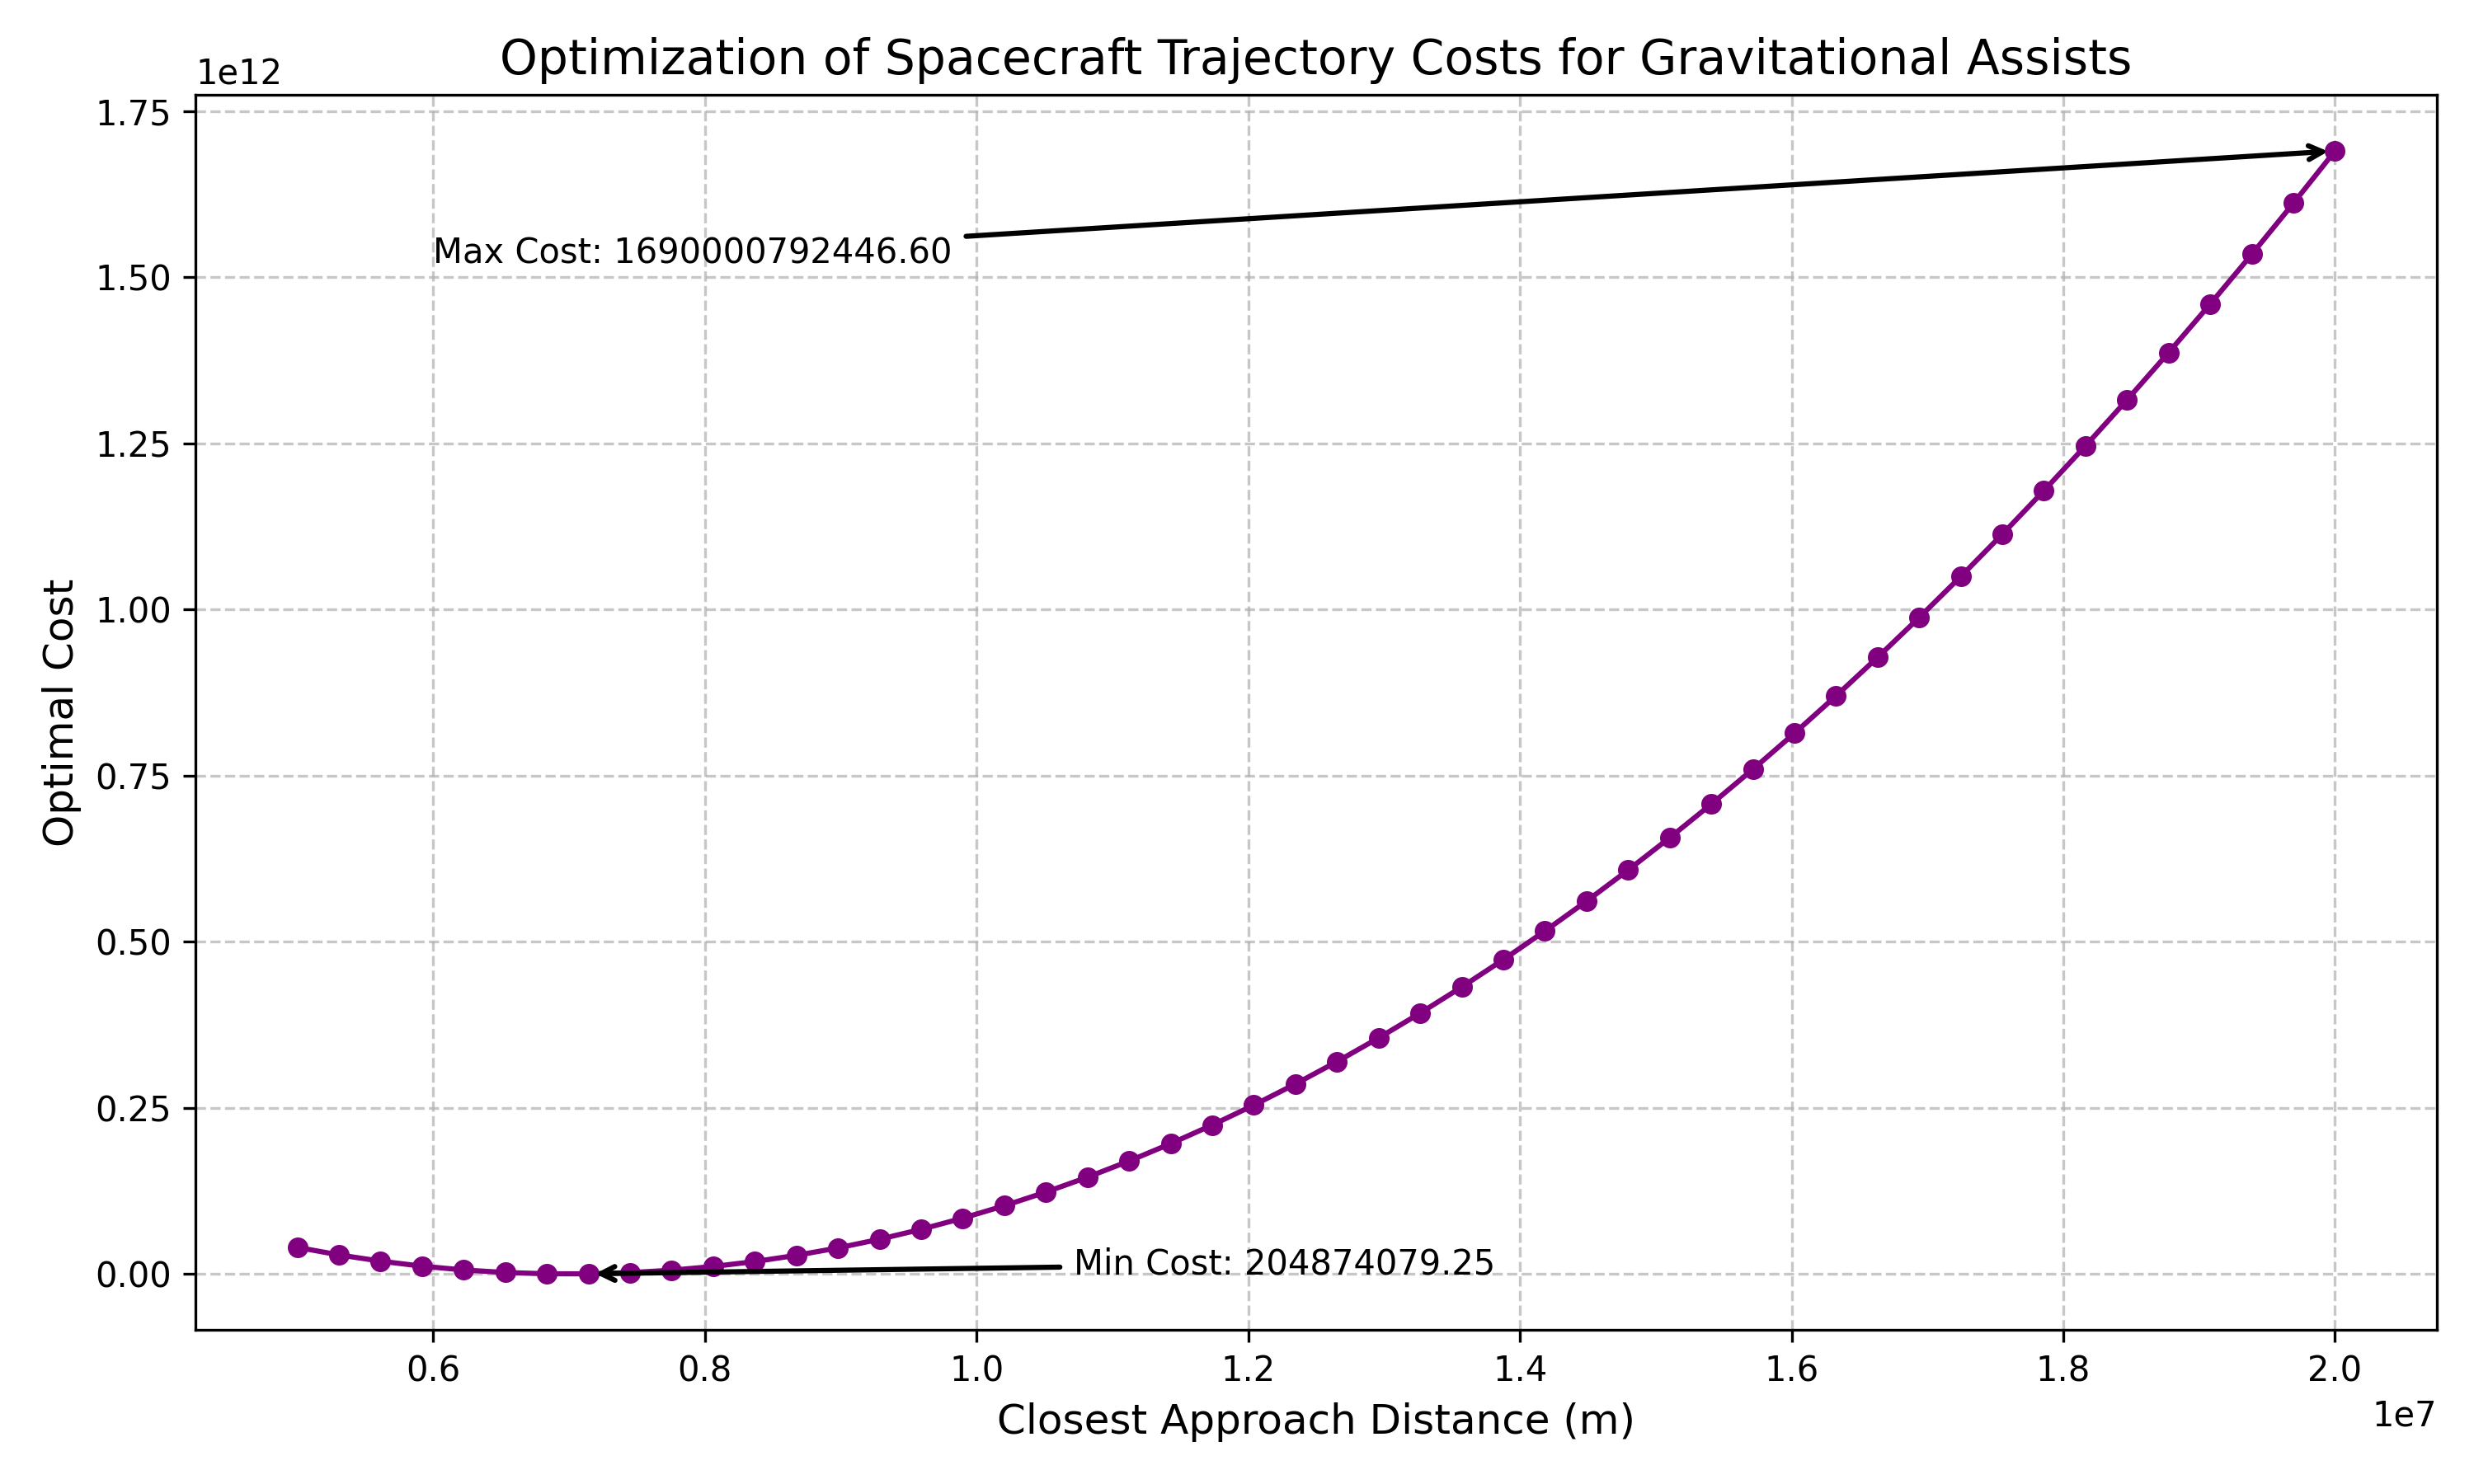
\includegraphics[width=\textwidth]{plots/optimize_trajectory_plot.png}%
\caption{Example plot of Optimize Trajectory.}%
\end{figure}

%
\clearpage%
\subsection{Code Listing}%
\label{subsec:CodeListing}%
\lstinputlisting[language=Python]{python_code/optimize_trajectory.py}

%
\newpage%
\section{Predator-Prey System}

\subsection{Introduction}

The predator-prey system is a set of differential equations known as the Lotka-Volterra equations, which describe the dynamics of biological systems in which two species interact: a prey and a predator.

\subsection{Variables}

\begin{itemize}
    \item $p_{\text{prey}}$: Population of prey at time $t$.
    \item $p_{\text{predator}}$: Population of predators at time $t$.
    \item $t$: Time variable.
    \item $\alpha$: Growth rate of the prey.
    \item $\beta$: Rate at which predators consume prey.
    \item $\delta$: Growth rate of predators due to consumption of prey.
    \item $\gamma$: Natural death rate of predators.
\end{itemize}

\subsection{Formulas}

\begin{align*}
    \frac{dp_{\text{prey}}}{dt} &= \alpha p_{\text{prey}} - \beta p_{\text{prey}} p_{\text{predator}} \\
    \frac{dp_{\text{predator}}}{dt} &= \delta p_{\text{prey}} p_{\text{predator}} - \gamma p_{\text{predator}}
\end{align*}%
\subsection{Example}

Consider a predator-prey system with the following parameters and initial conditions:

\begin{align*}
    \alpha &= 0.1 \quad \text{(prey growth rate)} \\
    \beta &= 0.02 \quad \text{(rate at which predators consume prey)} \\
    \delta &= 0.01 \quad \text{(rate at which prey consumption converts into predator growth)} \\
    \gamma &= 0.1 \quad \text{(predator death rate)} \\
    p_{\text{prey, initial}} &= 40 \quad \text{(initial population of prey)} \\
    p_{\text{predator, initial}} &= 9 \quad \text{(initial population of predators)}
\end{align*}

The time variable $t$ represents the temporal progression of the system:

\begin{align*}
    t &= [0, 200] \quad \text{(time points for simulation at intervals)}
\end{align*}

These equations describe how the populations of prey and predators change over time based on the initial conditions and parameters defined. The solution of these differential equations provides insights into the dynamics of the predator and prey populations within the specified time frame.%


\begin{figure}[H]%
\centering%
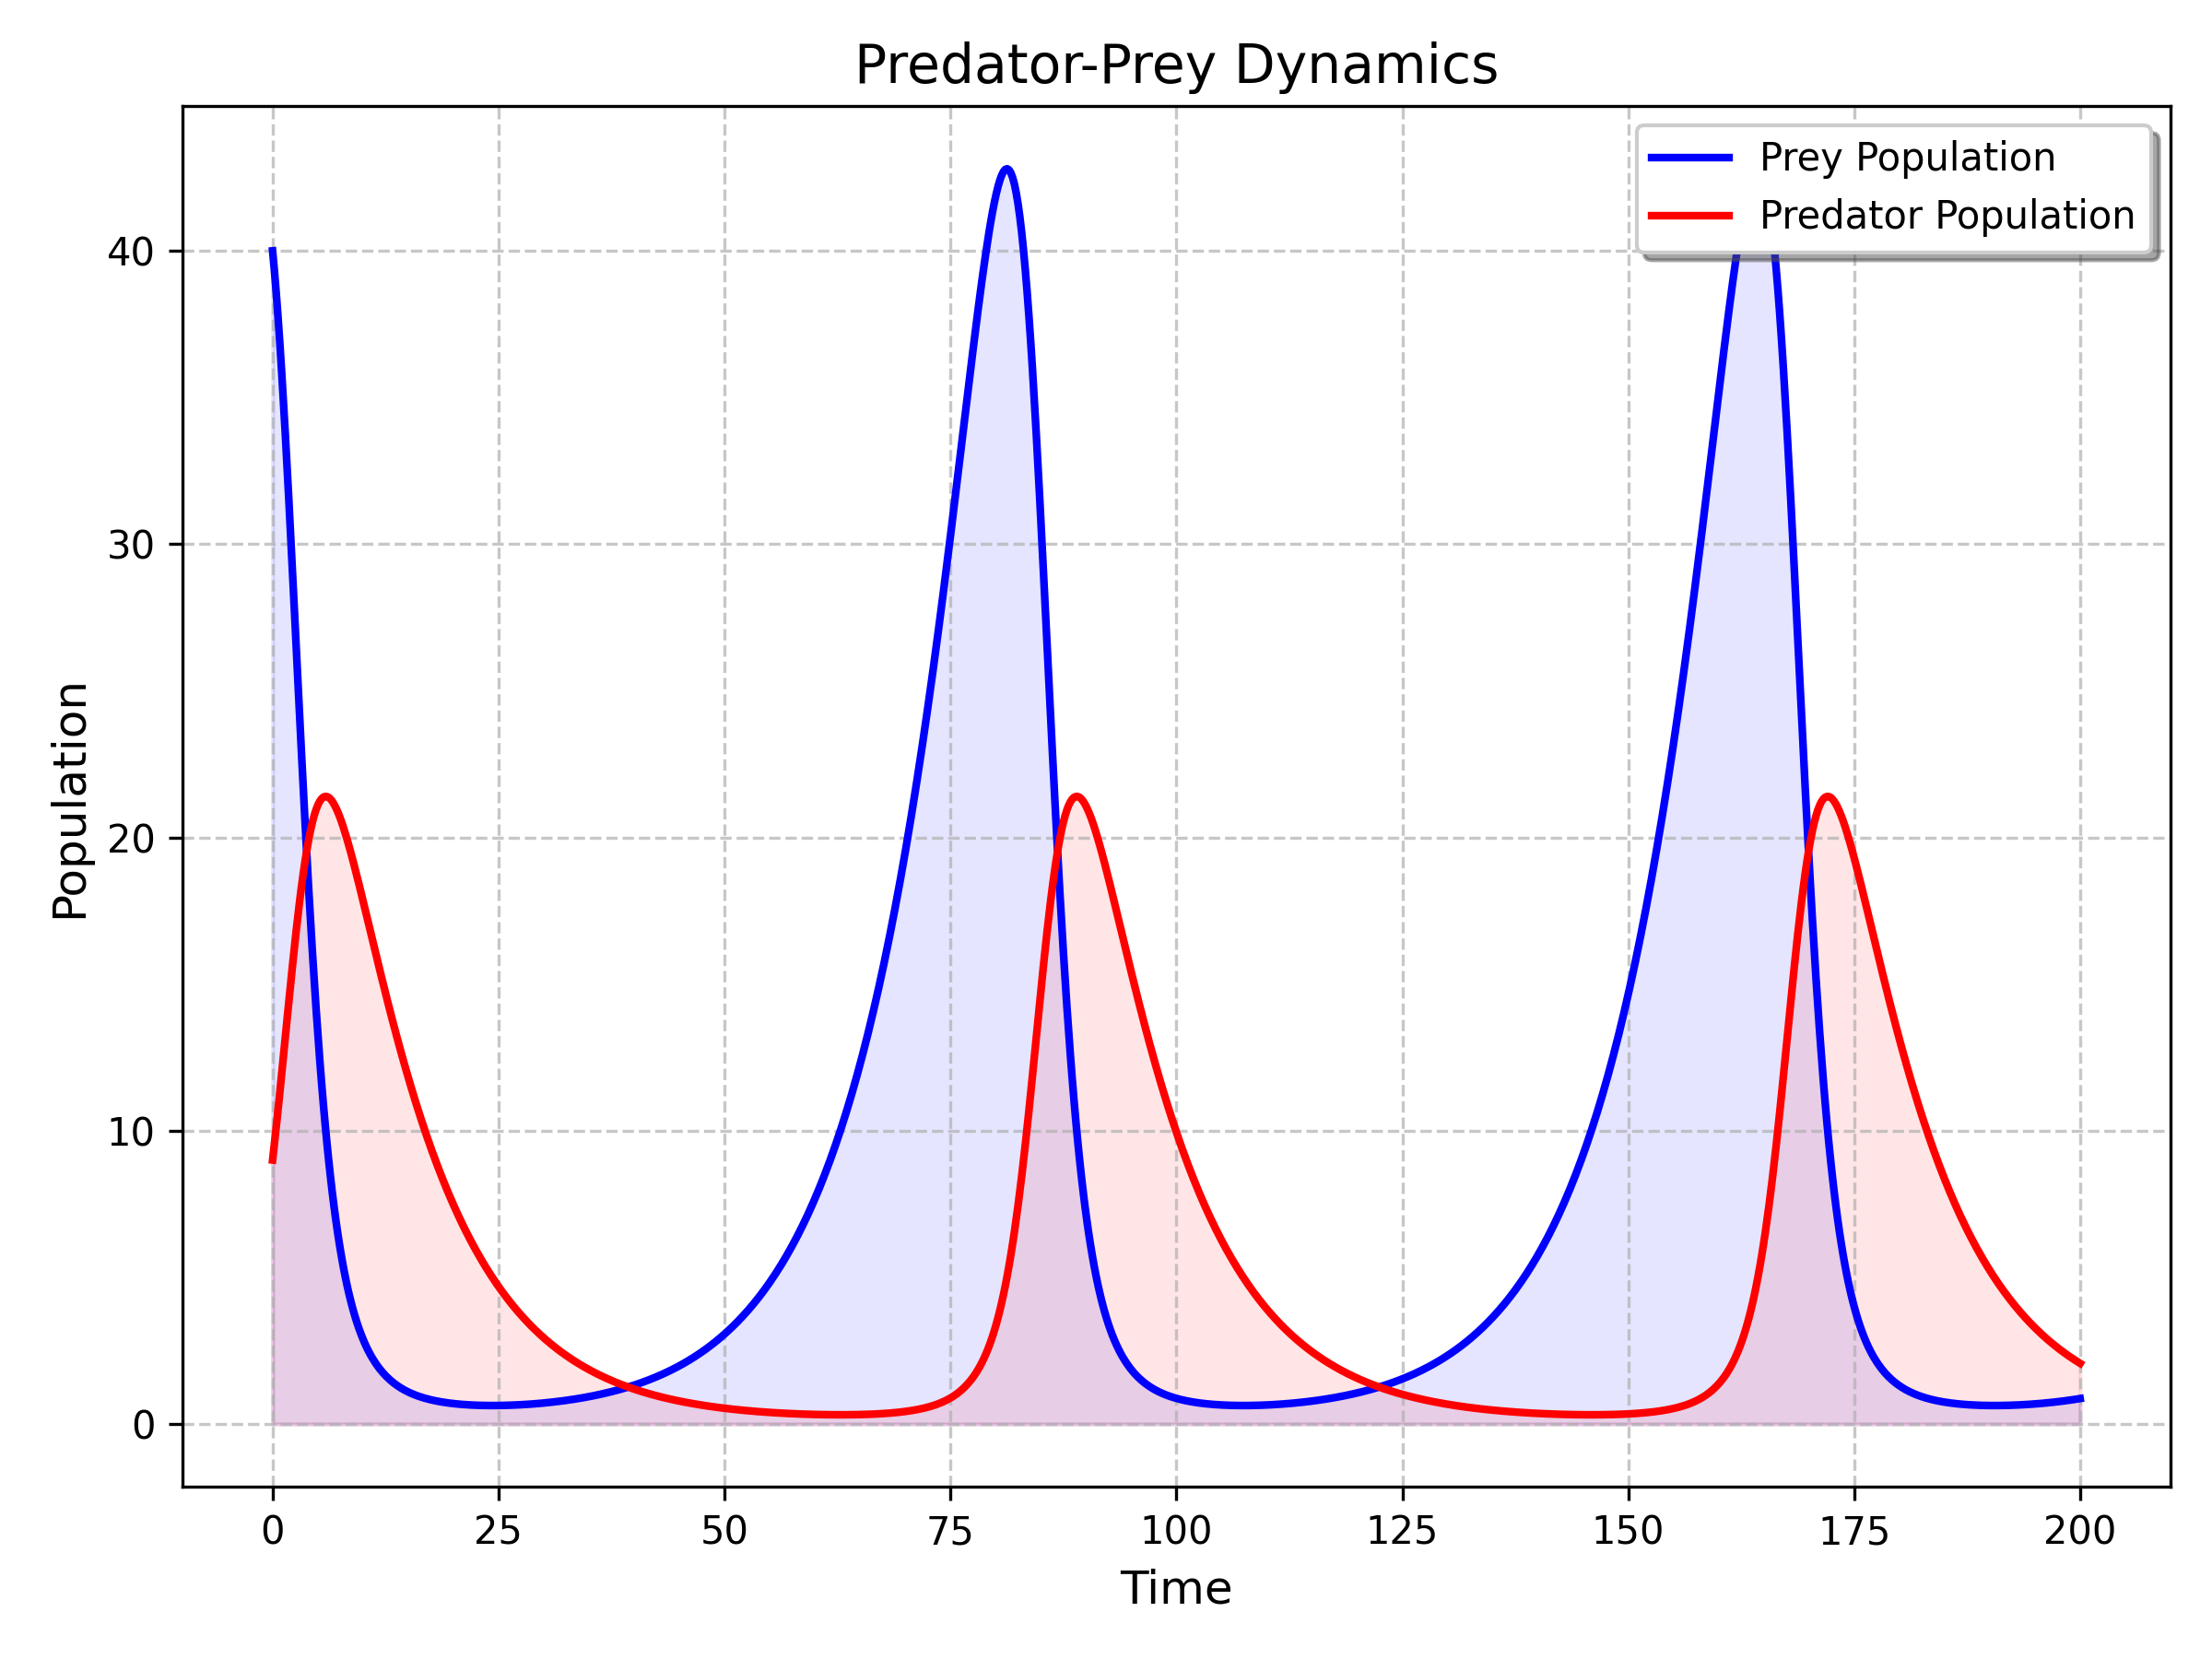
\includegraphics[width=\textwidth]{plots/predator_prey_system_plot.png}%
\caption{Example plot of Predator Prey System.}%
\end{figure}

%
\clearpage%
\subsection{Code Listing}%
\label{subsec:CodeListing}%
\lstinputlisting[language=Python]{python_code/predator_prey_system.py}

%
\newpage%
\section{Gravitational Assist Algorithm}

\subsection{Introduction}
This section outlines an algorithm for calculating the final velocity of a spacecraft after a gravitational assist with a planet. The calculation considers the initial velocities, masses, and distances involved.

\subsection{Variables}
\begin{itemize}
    \item $v_{\text{sc}}$: Initial velocity of the spacecraft in m/s.
    \item $v_{\text{p}}$: Velocity of the planet in m/s.
    \item $m_{\text{p}}$: Mass of the planet in kg.
    \item $d_{\text{closest}}$: Distance of closest approach in meters.
    \item $v_{\text{rel, init}}$: Relative initial velocity between spacecraft and planet.
    \item $v_{\infty}$: Velocity at infinity (far from the planet) after gravitational interaction.
    \item $v_{\text{final}}$: Spacecraft's final velocity after the gravitational assist.
    \item $G$: Gravitational constant, $6.67430 \times 10^{-11} \, \text{m}^3 \, \text{kg}^{-1} \, \text{s}^{-2}$.
\end{itemize}

\subsection{Formulas}
\begin{align*}
    v_{\text{rel, init}} &= |v_{\text{sc}} - v_{\text{p}}| \\
    v_{\infty} &= \sqrt{v_{\text{rel, init}}^2 + \frac{2 \cdot G \cdot m_{\text{p}}}{d_{\text{closest}}}} \\
    v_{\text{final}} &= \sqrt{v_{\text{sc}}^2 + 2 \cdot (v_{\infty}^2 - v_{\text{sc}} \cdot v_{\infty} \cdot \cos(\pi))}
\end{align*}%
\subsection{Example}
The following example demonstrates the calculation of the spacecraft's final velocity after a gravitational assist maneuver using specific initial conditions.

\begin{align*}
    &\text{Given}: \\
    &v_{\text{sc}} = 1.2 \times 10^4 \, \text{m/s}, \\
    &v_{\text{p}} = 2.4 \times 10^4 \, \text{m/s}, \\
    &m_{\text{p}} = 5.972 \times 10^{24} \, \text{kg}, \\
    &d_{\text{closest}} = 6.7 \times 10^6 \, \text{m}, \\
    \\
    &\text{First, find the relative initial velocity:} \\
    &v_{\text{rel, init}} = |v_{\text{sc}} - v_{\text{p}}| = |1.2 \times 10^4 - 2.4 \times 10^4| \, \text{m/s}. \\
    \\
    &\text{Next, calculate the velocity at infinity:} \\
    &v_{\infty} = \sqrt{v_{\text{rel, init}}^2 + \frac{2 \cdot G \cdot m_{\text{p}}}{d_{\text{closest}}}}, \\
    &\text{where } G = 6.67430 \times 10^{-11} \, \text{m}^3 \, \text{kg}^{-1} \, \text{s}^{-2}. \\
    \\
    &\text{Finally, compute the spacecraft's final velocity:} \\
    &v_{\text{final}} = \sqrt{v_{\text{sc}}^2 + 2 \cdot (v_{\infty}^2 - v_{\text{sc}} \cdot v_{\infty} \cdot \cos(\pi))}.
\end{align*}%


\begin{figure}[H]%
\centering%
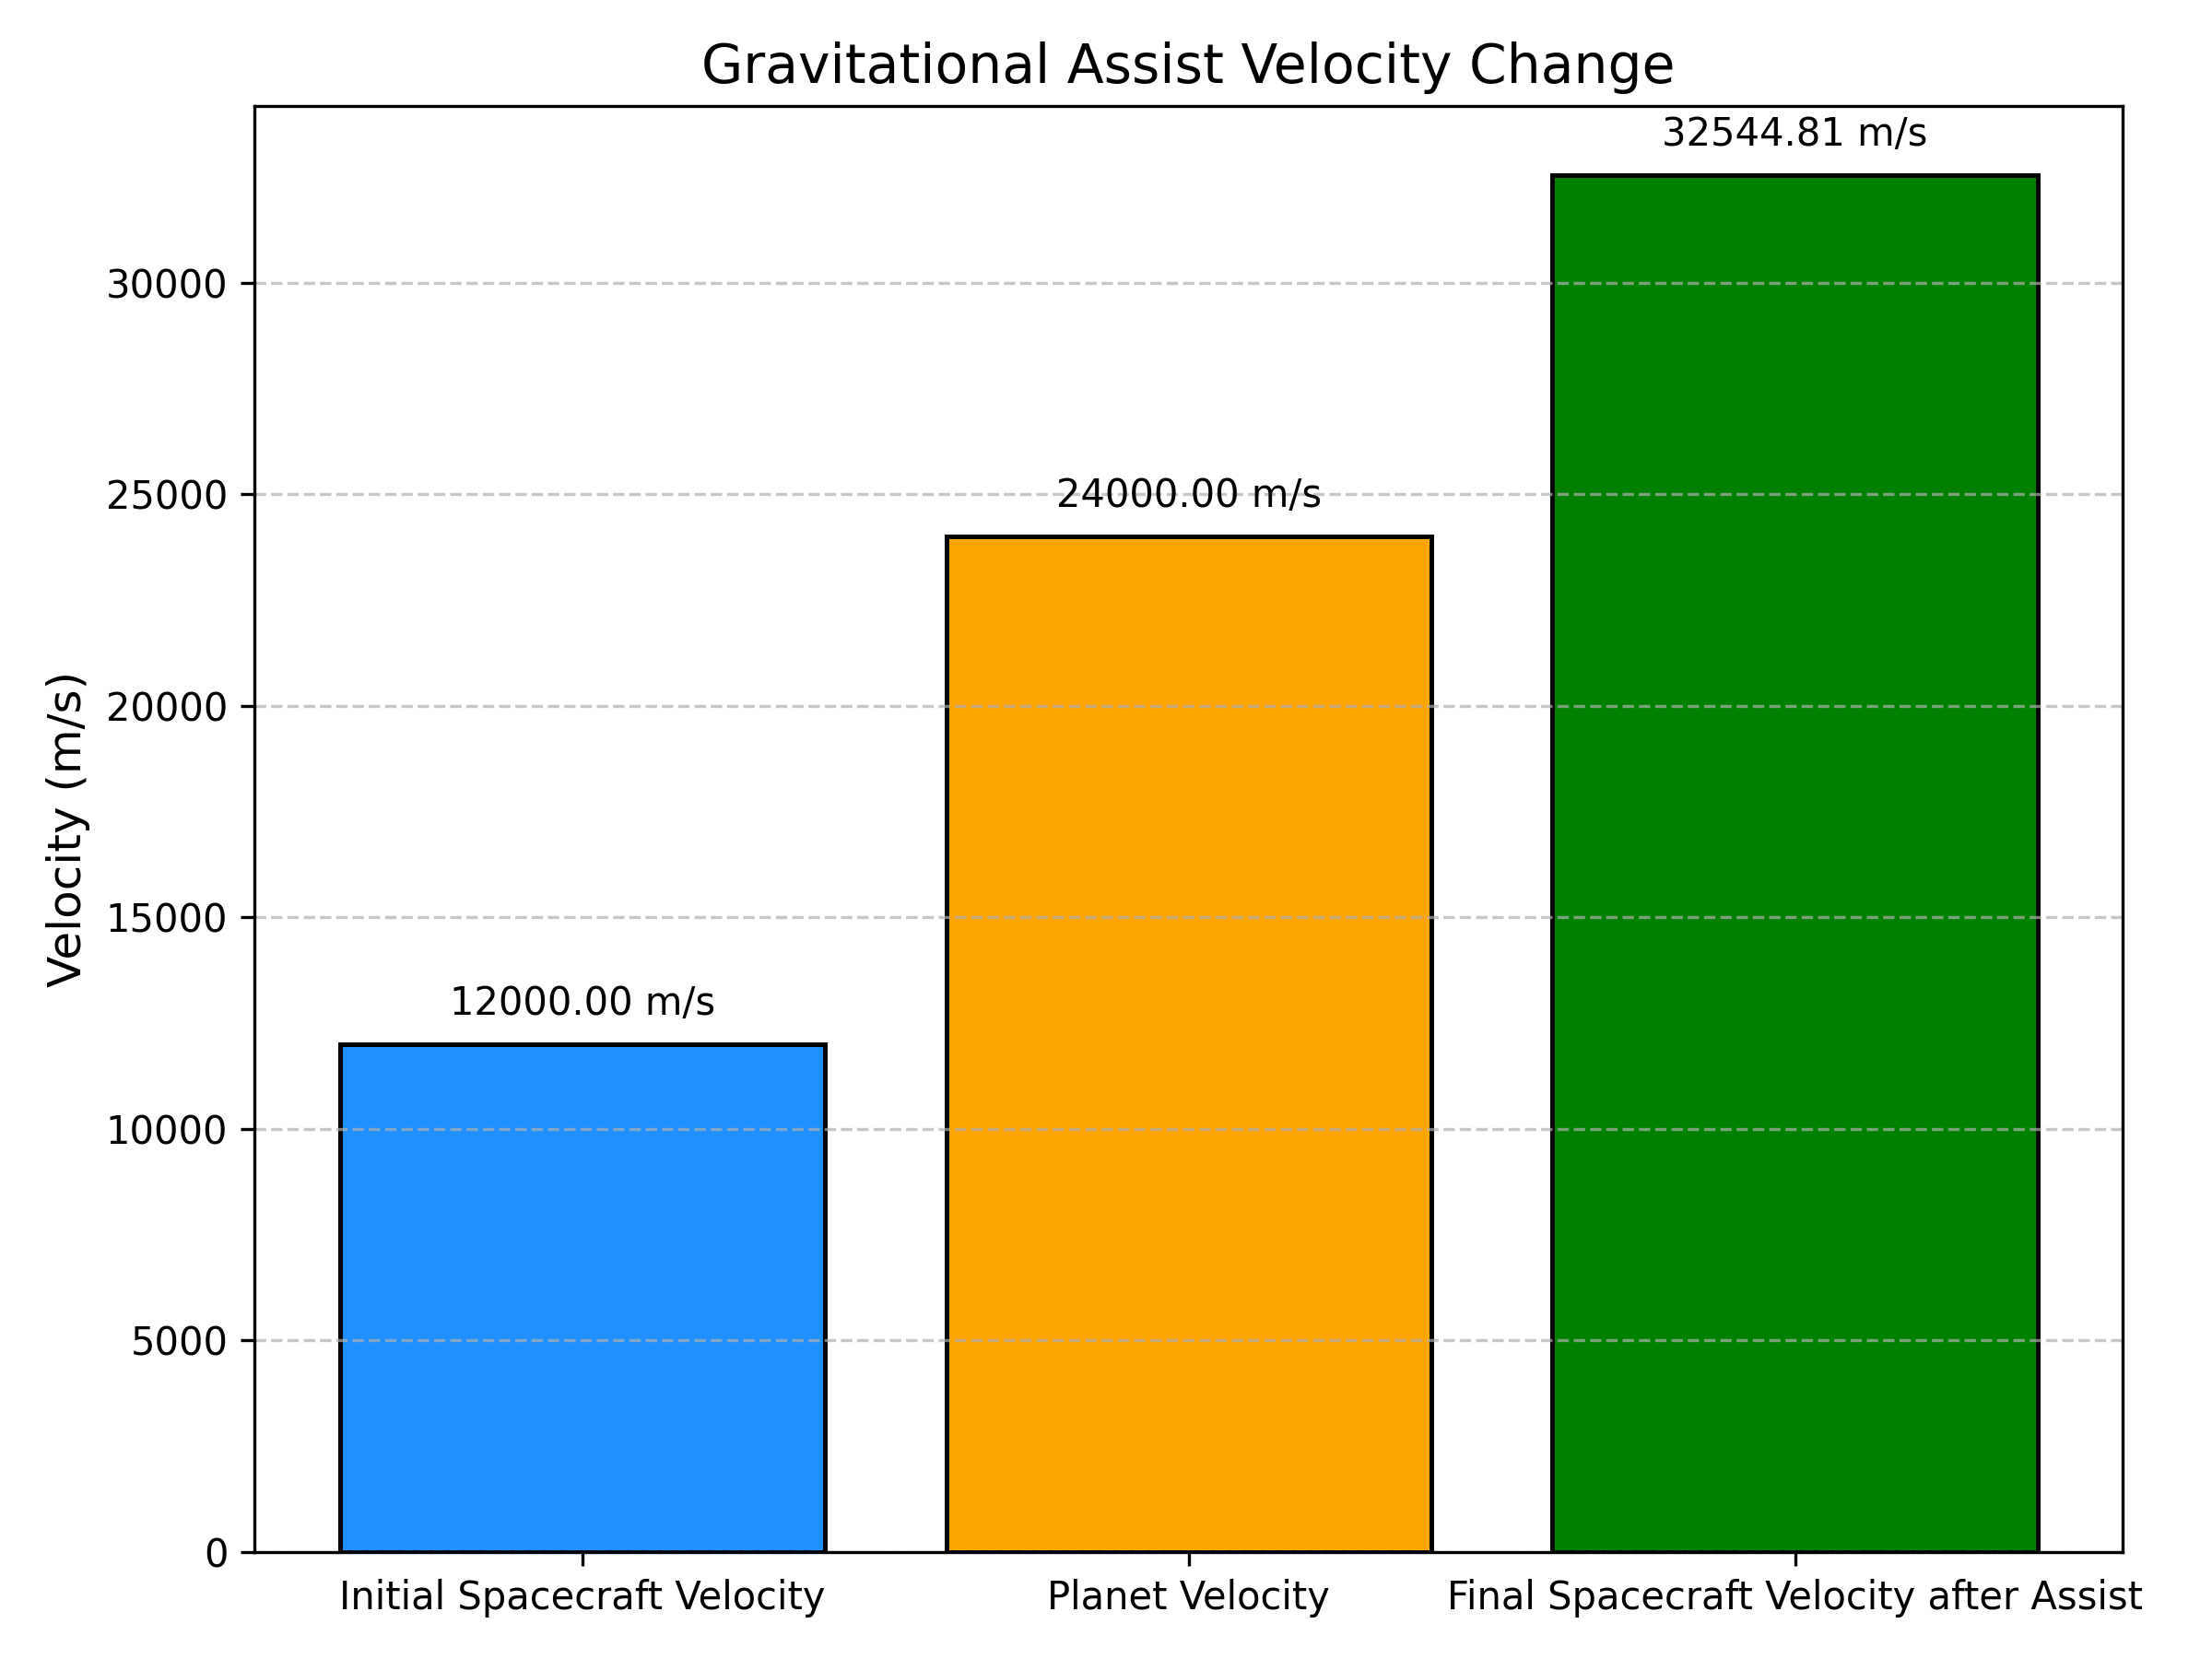
\includegraphics[width=\textwidth]{plots/gravitational_assist_plot.png}%
\caption{Example plot of Gravitational Assist.}%
\end{figure}

%
\clearpage%
\subsection{Code Listing}%
\label{subsec:CodeListing}%
\lstinputlisting[language=Python]{python_code/gravitational_assist.py}

%
\newpage%
\section{Hohmann Transfer Orbit Calculation}

\subsection{Introduction} 
The Hohmann transfer algorithm calculates the velocity changes (delta-v) required to transfer a spacecraft from Earth's orbit to Mars's orbit. This is achieved through the use of gravitational interactions, specifically the Sun's gravitational influence.

\subsection{Variables}

\begin{itemize}
    \item $r_{\text{earth}}$: Radius of Earth's orbit around the Sun in meters.
    \item $r_{\text{mars}}$: Radius of Mars's orbit around the Sun in meters.
    \item $\mu_{\text{sun}}$: Gravitational constant for the Sun in m$^3$/s$^2$.
    \item $v_{\text{earth}}$: Velocity of Earth in its orbit.
    \item $v_{\text{mars}}$: Velocity of Mars in its orbit.
    \item $a_{\text{transfer}}$: Semi-major axis of the Hohmann transfer orbit.
    \item $v_{\text{transfer\_earth}}$: Velocity required at Earth for the transfer orbit.
    \item $v_{\text{transfer\_mars}}$: Velocity required at Mars for the transfer orbit.
    \item $\Delta v_{\text{earth}}$: Delta-v required to escape Earth's orbit and enter the transfer orbit.
    \item $\Delta v_{\text{mars}}$: Delta-v required to enter Mars's orbit from the transfer orbit.
    \item $\Delta v_{\text{total}}$: Total delta-v for the entire transfer.
\end{itemize}

\subsection{Formulas}

\begin{align*}
    \mu_{\text{sun}} &= 1.32712440018 \times 10^{20} \, \text{m}^3/\text{s}^2 \\
    v_{\text{earth}} &= \sqrt{\frac{\mu_{\text{sun}}}{r_{\text{earth}}}} \\
    v_{\text{mars}} &= \sqrt{\frac{\mu_{\text{sun}}}{r_{\text{mars}}}} \\
    a_{\text{transfer}} &= \frac{r_{\text{earth}} + r_{\text{mars}}}{2} \\
    v_{\text{transfer\_earth}} &= \sqrt{\frac{2\mu_{\text{sun}}}{r_{\text{earth}}} - \frac{\mu_{\text{sun}}}{a_{\text{transfer}}}} \\
    v_{\text{transfer\_mars}} &= \sqrt{\frac{2\mu_{\text{sun}}}{r_{\text{mars}}} - \frac{\mu_{\text{sun}}}{a_{\text{transfer}}}} \\
    \Delta v_{\text{earth}} &= v_{\text{transfer\_earth}} - v_{\text{earth}} \\
    \Delta v_{\text{mars}} &= v_{\text{mars}} - v_{\text{transfer\_mars}} \\
    \Delta v_{\text{total}} &= \lvert \Delta v_{\text{earth}} \rvert + \lvert \Delta v_{\text{mars}} \rvert
\end{align*}%
\subsection{Example}

To demonstrate the Hohmann transfer orbit calculation, consider the following scenario:

\begin{align*}
    r_{\text{earth}} &= 1.496 \times 10^{11} \, \text{m} \\
    r_{\text{mars}} &= 2.279 \times 10^{11} \, \text{m} \\
    \Delta v_{\text{earth}}, \Delta v_{\text{mars}}, \Delta v_{\text{total}} &= \text{calculate\_hohmann\_transfer}(r_{\text{earth}}, r_{\text{mars}})
\end{align*}

To visualize the orbits involved in the transfer, consider the following coordinates:

1. Earth's orbit around the Sun is circular, with coordinates \((x, y)\) given by:
   \begin{align*}
       x_{\text{earth}} &= r_{\text{earth}} \cdot \cos(\theta) \\
       y_{\text{earth}} &= r_{\text{earth}} \cdot \sin(\theta)
   \end{align*}

2. Similarly, Mars's orbit coordinates are given by:
   \begin{align*}
       x_{\text{mars}} &= r_{\text{mars}} \cdot \cos(\theta) \\
       y_{\text{mars}} &= r_{\text{mars}} \cdot \sin(\theta)
   \end{align*}

For the transfer orbit:

- The semi-major axis \(a_{\text{transfer}}\) and eccentricity \(e_{\text{transfer}}\) are calculated as follows:
  \begin{align*}
      a_{\text{transfer}} &= \frac{r_{\text{earth}} + r_{\text{mars}}}{2} \\
      e_{\text{transfer}} &= \frac{r_{\text{mars}} - r_{\text{earth}}}{r_{\text{earth}} + r_{\text{mars}}}
  \end{align*}

- The coordinates \((x, y)\) for the Hohmann transfer orbit are:
  \begin{align*}
      x_{\text{transfer}} &= a_{\text{transfer}} \cdot (\cos(\theta) - e_{\text{transfer}}) \\
      y_{\text{transfer}} &= a_{\text{transfer}} \cdot \sqrt{1 - e_{\text{transfer}}^2} \cdot \sin(\theta)
  \end{align*}

The total velocity change \(\Delta v_{\text{total}}\) required for the transfer orbit is given by:
\begin{align*}
    \Delta v_{\text{total}} &= \Delta v_{\text{earth}} + \Delta v_{\text{mars}}
\end{align*}%


\begin{figure}[H]%
\centering%
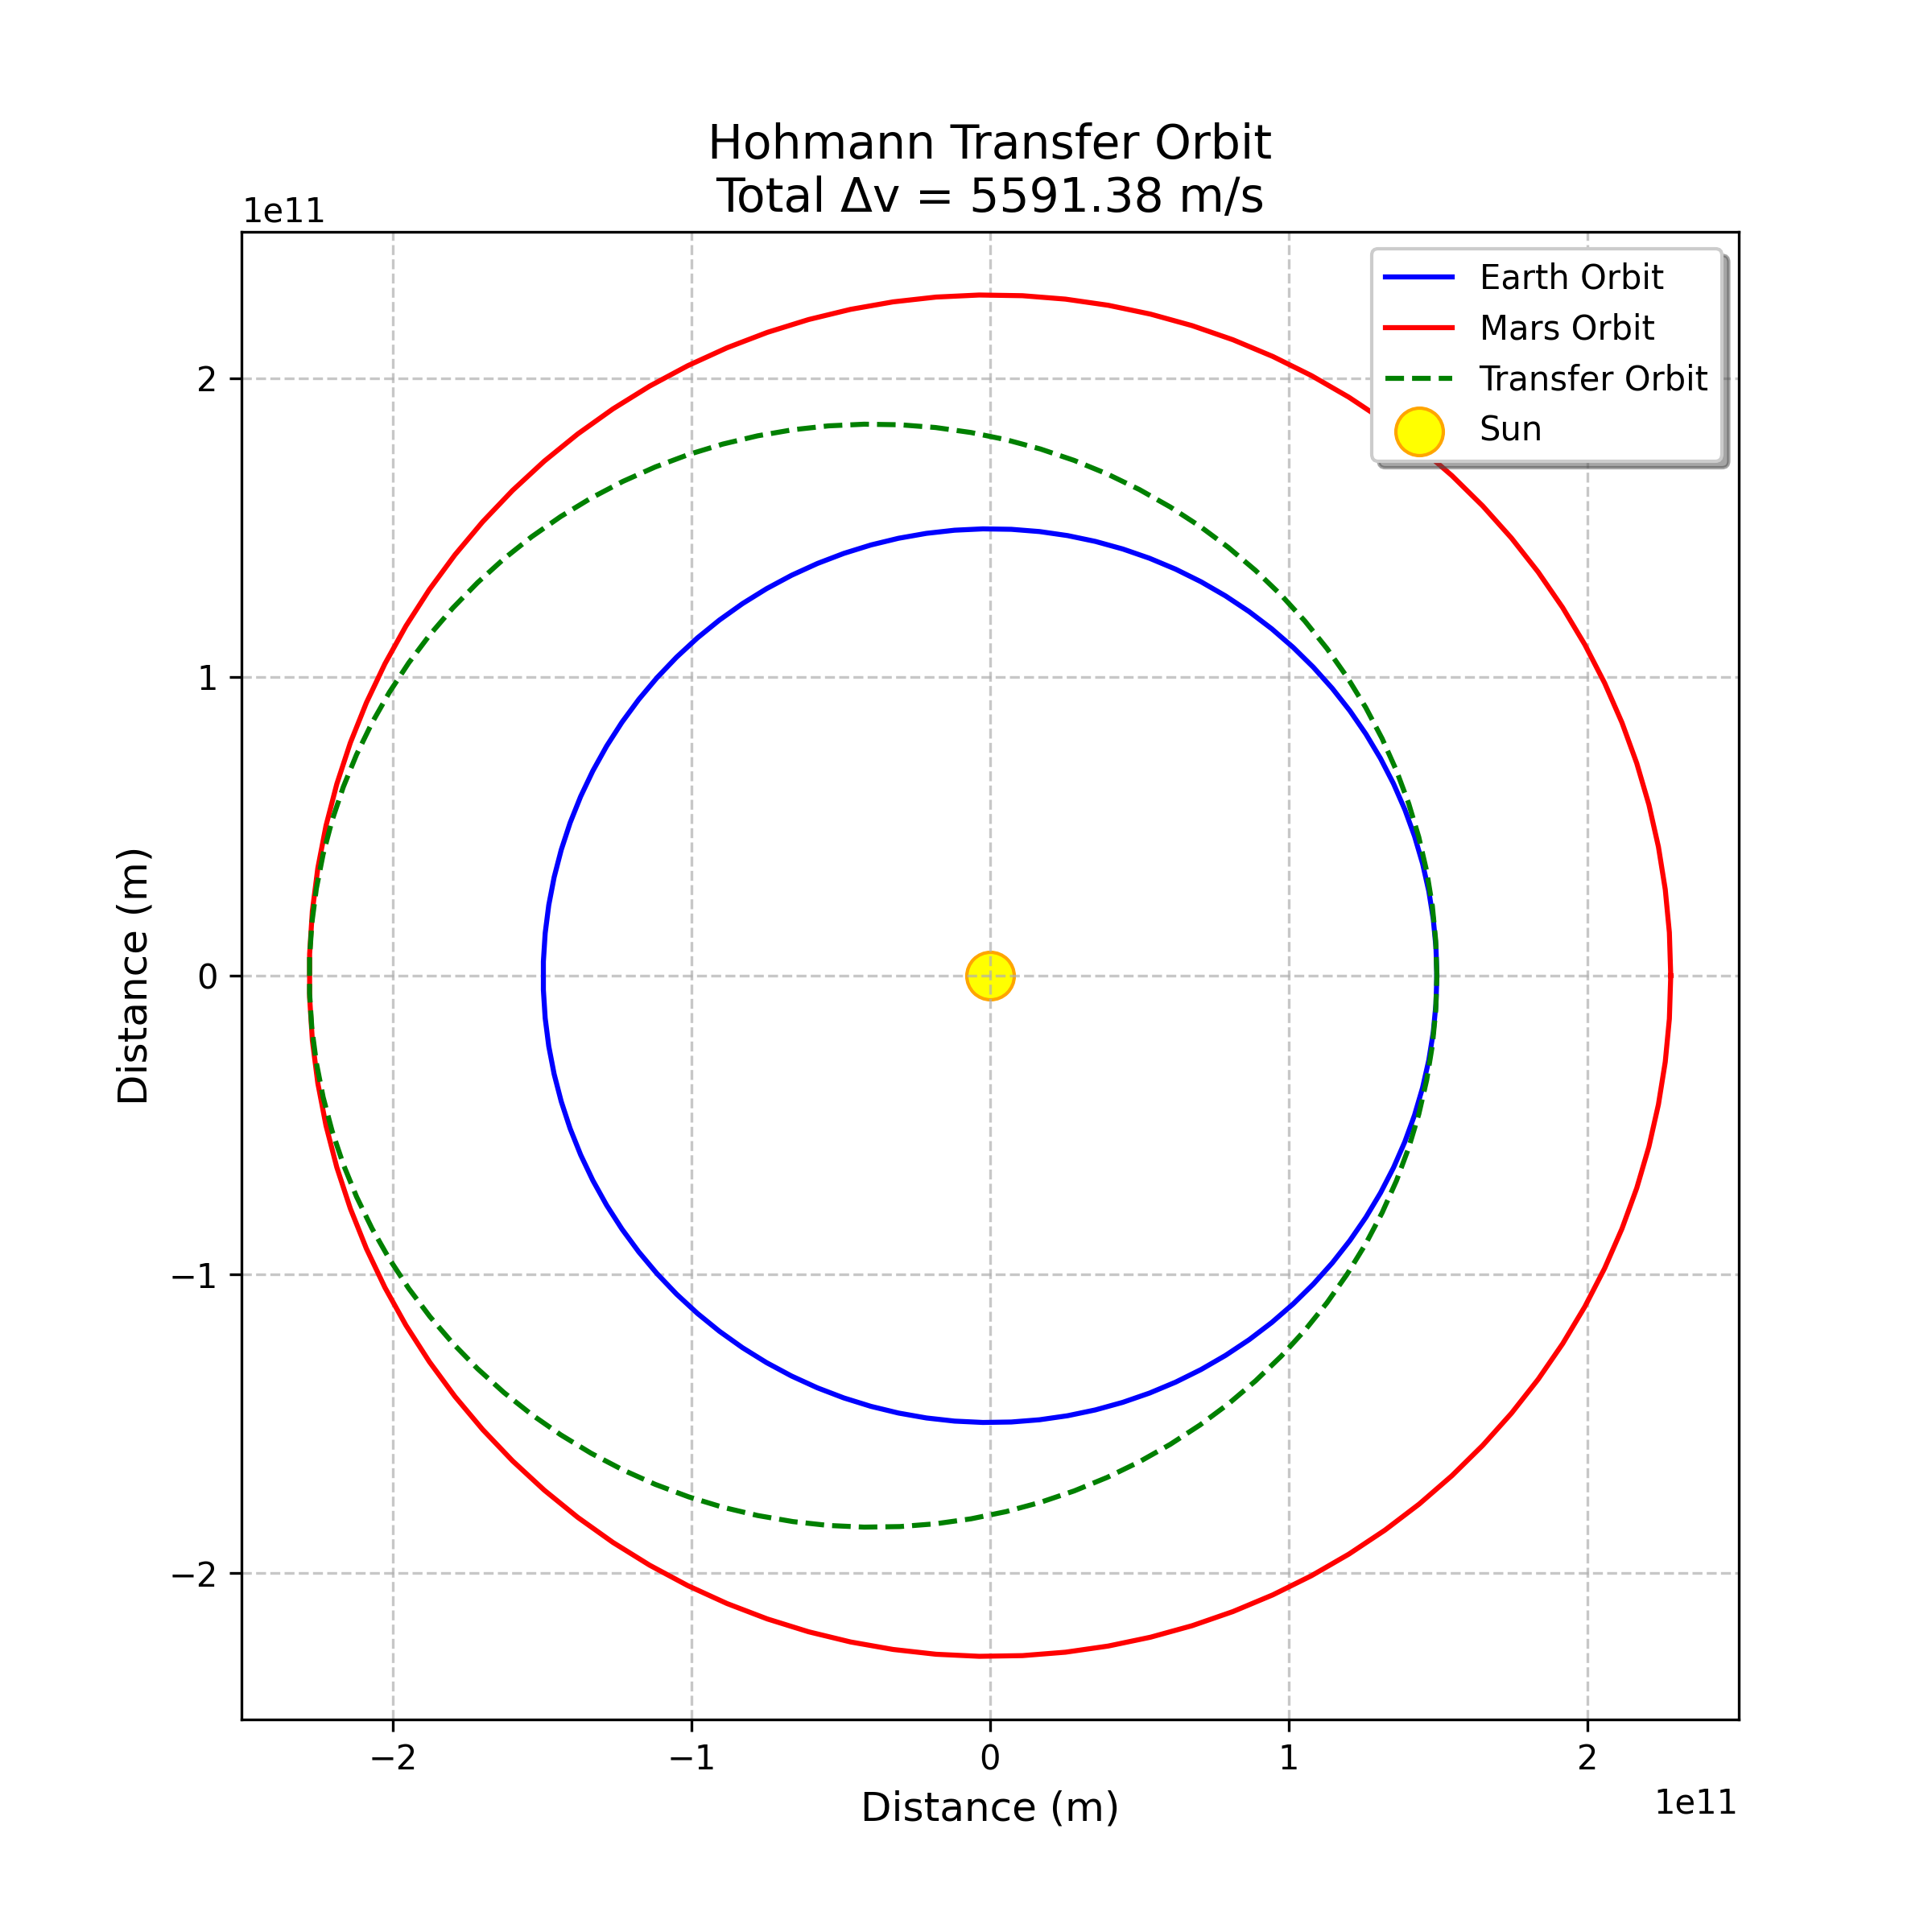
\includegraphics[width=\textwidth]{plots/calculate_hohmann_transfer_plot.png}%
\caption{Example plot of Calculate Hohmann Transfer.}%
\end{figure}

%
\clearpage%
\subsection{Code Listing}%
\label{subsec:CodeListing}%
\lstinputlisting[language=Python]{python_code/calculate_hohmann_transfer.py}

%
\end{document}